Matheuristics refers to the integration of Mathematical Programming and problem-specific heuristics to develop hybrid algorithms that leverage the strengths of both approaches. Many real-world optimization problems are computationally challenging and may not be efficiently solvable using exact mathematical programming approaches alone. This is where heuristics come into play. Heuristics are approximate methods that trade optimality for computational efficiency. They aim to quickly find good solutions by leveraging problem-specific knowledge, rules of thumb, or iterative improvement techniques.
The combination of mathematical programming and heuristics in matheuristics allows for a powerful approach to tackle complex optimization problems, providing a good balance between solution quality and computational efficiency. It is particularly useful for problems, such as TSP, where finding exact optimal solutions is infeasible or time-consuming, but good-quality solutions are still desired within a reasonable amount of time.
In the following section we present two of such techniques, that are hard fixing and local branching.

\section{Hard Fixing}
Hard-fixing matheuristics is a specific approach that sets the value of certain decision variables to a specific value and then tries to solve the new simplified problem with the remaining variables. By fixing variables, the problem size is reduced, and the solver can focus on finding a solution in a smaller search space.\\
In our case we fix the decision variables that indicate if an edge is selected or not. We fix those variables as selected, and then we try to solve the new problem with the MIP solver.\\
Once the solution is found, the fixed variables are unfixed, and the procedure restarts until a given time limit is reached.
We first find an initial solution to the problem using the greedy heuristic. Then we construct the basic mathematical model, without the SEC. For every edge e that belongs to the solution provided by the heuristic, we choose with a probability equal to \textit{p} $\in$(0,1) if the edge has to be fixed or not. To fix an edge we simply set the lower bound equal to 1 to the variable corresponding to it. At this point the user-cut callback is used to solve the problem.\\ 
Once a solution has been found, all the lower bounds are set to 0, and from this new solution with the same procedure as before new edges are fixed, and so on until the given time limit is reached.\\
The performance of this method is highly conditioned by the type of the initial solution: if the initial solution is not very good, there is the risk that this approach will get stuck on a non-optimal solution.


\begin{algorithm}
    \caption{Hard Fixing}\label{algo:HardFixing}
    \begin{algorithmic}[1]
    \Require $G = (V,E), c:E \to \mathbb{R}^+$
    \Ensure $\text{sub optimal TSP solution}$

    \State $solution \gets$ greedy()
    \State $cost \gets $ cost(solution)
    \State $*$ Build basic TSP model in CPLEX $*$



    \While{$ !time\textunderscore expired  $}
    \ForEach {edge e$\in$ solution}
    \State $*$ fix e with probability p $*$
    \EndFor
    \State $solution \gets$ findNewSolution()
    \If{cost(solution) < cost(best\textunderscore solution)}
    \State $ best\textunderscore solution \gets$ solution
    \EndIf
    \State $*$ unfix all variables $*$
    \EndWhile

    \end{algorithmic}
\end{algorithm}

\subsection{Tuning of HardFixing}
An essential aspect of our hard fixing method's implementation lies in the parameter that governs the probability of fixing a specific edge. Consequently, we have embarked on tuning this parameter to achieve enhanced performance.
\\
Figure \ref{fig:hard} illustrates the diverse probabilities tested in the matheuristic. The values shown in the figure represent the true probabilities divided by ten. Notably, the value 8 demonstrates superior performance, corresponding to selecting 80\% of the edges from the previous solution.
\begin{figure}[!h]
    \centering
    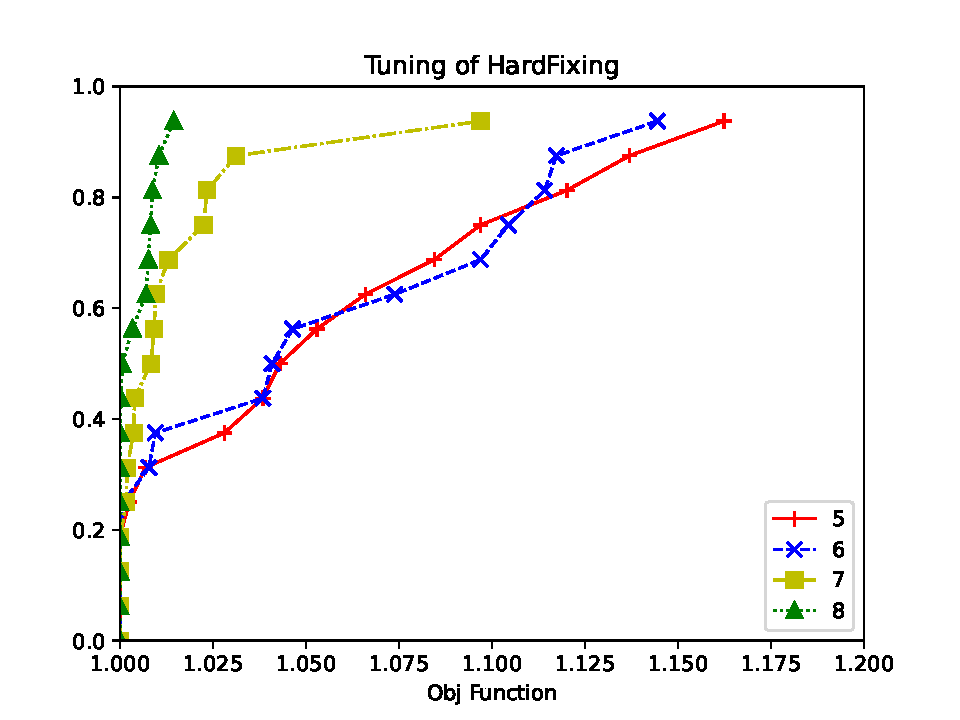
\includegraphics[width=\textwidth]{images/hard.pdf}
    \caption{Tuning of probability in HardFixing}
    \label{fig:hard}
\end{figure}

\section{Local Branching}

The Local Branching or soft fixing, is a matheuristic proposed by M. Fischetti and A. Lodi \cite{fischetti2003local}, that tries to improve the performance of the Hard-fixing matheuristics.\\
A critical point of hard-fixing consists in the choice of the variables that have to be fixed at each step. So, to try to solve this issue, soft fixing requires that a given number of variables have to be fixed, but unlike the hard-fixing method, it doesn’t choose them explicitly. In Local Branching this operation is performed by adding a new constraint that forces the solver to maintain a certain number of variables to the previous value. In our case we add a constraint that informs the solver that a given number of edges have to be maintained. \\

\begin{algorithm}[h!]
    \caption{Local Branching}\label{algo:SoftFixing}
    \begin{algorithmic}[1]
    \Require $G = (V,E), c:E \to \mathbb{R}^+$
    \Ensure $\text{sub optimal TSP solution}$

    \State $solution \gets$ greedy()
    \State $cost \gets $ cost(solution)
    \State $*$ Build basic TSP model in CPLEX $*$



    \While{$ !time\textunderscore expired  $}
    \State $*$ add constraint \ref{eq:localBranch} $*$
    \State $solution \gets$ findNewSolution()
    \If{cost(solution) < cost(best\textunderscore solution)}
    \State $ best\textunderscore solution \gets$ solution
    \ElsIf{not improvement for a certain number of iteration}
    \State $*$ change parameter k $*$
    \EndIf
    \State $*$ remove constraint \ref{eq:localBranch} $*$
    \EndWhile

    \end{algorithmic}
\end{algorithm}

The main idea behind this approach is the Hamming distance. This particular distance measures the number of positions at which the corresponding symbols are different. It can be used to calculate the “distance” between two vectors. \\
We can apply this concept to the vector that represents the solution of a TSP instance. This solution can be seen as a binary vector, of length |E|, where each element is set to 1 if the corresponding edge is part of the solution and 0 otherwise. So given two vectors that corresponds to two different solutions of the same TSP instance, the Hamming distance between the two array can be formulated as:
\begin{equation}
   H(x,x^*)= \sum_{e\in E: x_e^*=1}^{}(1-x_e) + \sum_{e\in E: x_e^*=0}^{}x_e
\end{equation}
The first term counts the number of flipped 1’s, and the second counts the number of flipped 0’s. \\
Now looking at the form of the solution provided by the TSP solver, it is possible to add a new constraint that limits the hamming distance between the old and the new solution:

\begin{equation}\label{eq:hamming}
    \sum_{e\in E: x_e^*=1}^{}(1-x_e) + \sum_{e\in E: x_e^*=0}^{}x_e \leq r
\end{equation}
We know that a valid TSP solution has a number of edges equal to n (number of nodes), and the number of flipped 0’s is the same as the flipped 1’s . So applying these knowledges to the \ref{eq:hamming} equation and with the aid of some algebra tricks it can be reformulated as:
\begin{equation}\label{eq:localBranch}
    \sum_{e\in E: x_e^*=1}^{}x_e \geq n-k
\end{equation}
where k=r/2.
\\
In our specific implementation the parameter k is changed every time the solver is stuck in the same solution. \\
In Algorithm \ref{algo:SoftFixing} too, the initial solution is provided by the greedy heuristic, and from this start configuration the solver at each iteration tries to improve the incumbent adding the constraint \ref{eq:localBranch}, until the time limit is reached.




\subsection{Tuning of Local Branching}
In this specific case, our focus was on the algorithm's behavior when it repeatedly produces the same solution with a fixed value of ``k" in constraint \ref{eq:localBranch}. To address this, we fine-tuned the number of iterations the algorithm should execute without any improvement. Once this threshold is reached, the algorithm automatically adjusts the value of ``k". Figure \ref{fig:soft} provides insight into our findings, showing that setting the number of iterations without improvements to 5 results in optimal performance.
\begin{figure}[!h]
    \centering
    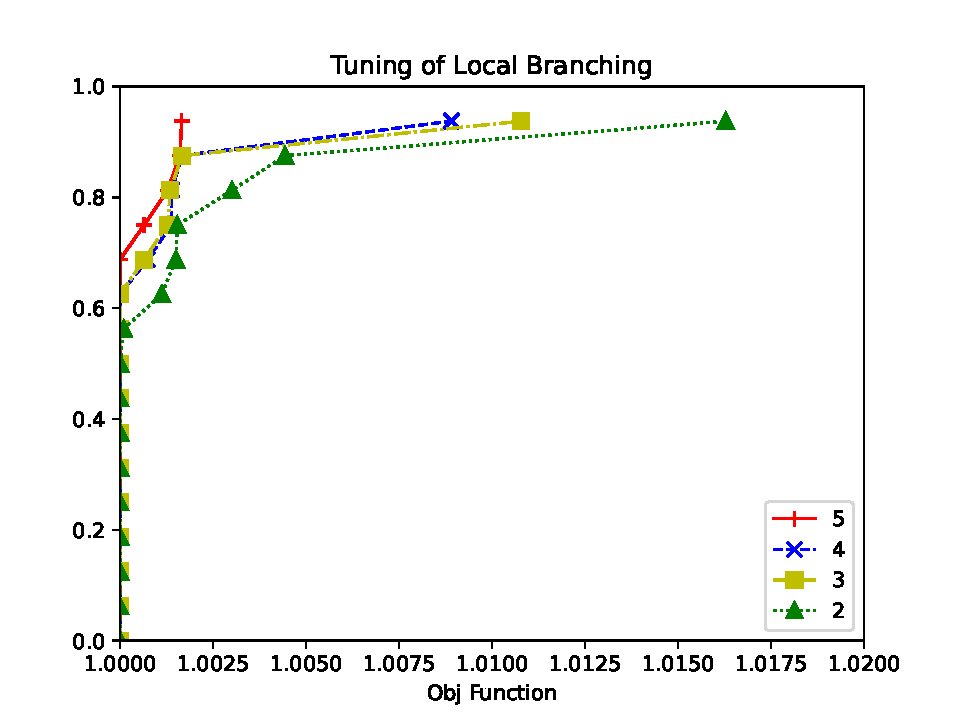
\includegraphics[width=\textwidth]{images/soft.pdf}
    \caption{Tuning of number of non improvement iteration before to change the value of k in Local Branching}
    \label{fig:soft}
\end{figure}


\section{Comparison of Matheuristics}

We tested the HardFixing Algorithm and the Local Branching Algorithm over the same instances, running for the same amount of time per instance. Both Figure \ref{fig:hs} and Table \ref{table:math} shows how they performs identically in more than 50\% of the instances, returning the same correct value. Overall HardFixing is by far the best one, since it provides stronger constraints and leads to more precise solutions. 

\begin{figure}[!h]
    \centering
    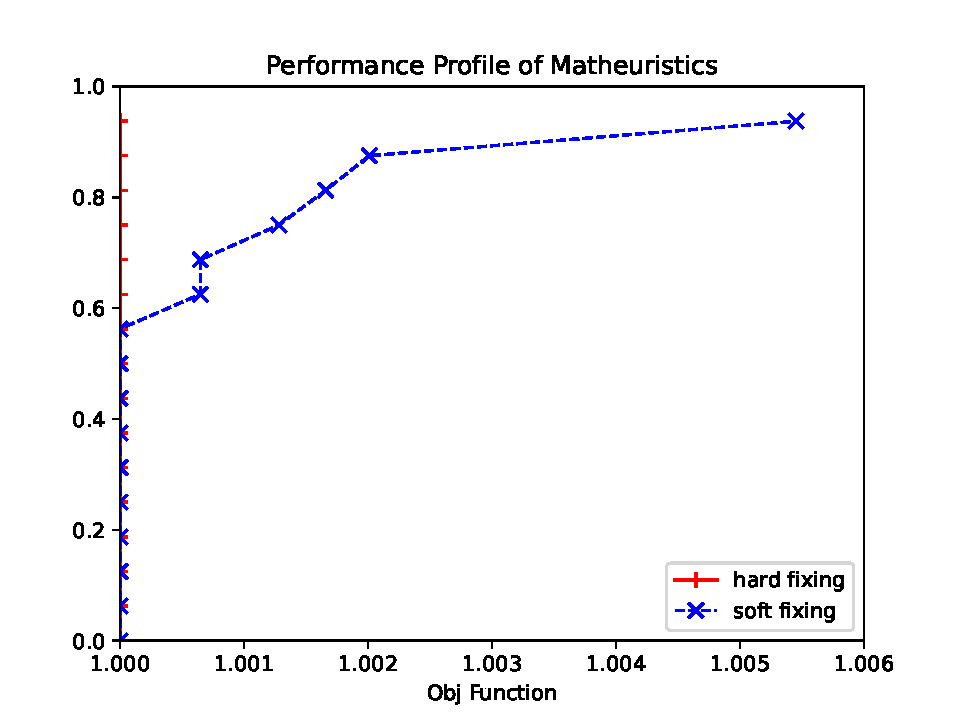
\includegraphics[width=\textwidth]{images/hs.pdf}
    \caption{Performance Profile of Matheuristics}
    \label{fig:hs}
\end{figure}

\begin{table}[!h]
    \centering
    \begin{tabular}{lcc}
    \cline{2-3}
                & \textbf{hard fixing} & \textbf{soft fixing} \\ \hline
    att48.tsp   & 10601.127450         & 10601.127450         \\
    att532.tsp  & 28212.391348         & 28248.540350         \\
    d493.tsp    & 35605.036596         & 35676.629322         \\
    d657.tsp    & 50855.493487         & 50855.493487         \\
    dsj1000.tsp & 21619342.0      & 21619342.0      \\
    lin318.tsp  & 42649.518313         & 42649.518313         \\
    p654.tsp    & 40251.581798         & 40251.581798         \\
    pcb442.tsp  & 51328.083821         & 51328.083821         \\
    pr1002.tsp  & 284653.597388        & 286205.676140        \\
    pr439.tsp   & 110741.414203        & 110741.414203        \\
    rat575.tsp  & 6960.514805          & 6965.028779          \\
    rat783.tsp  & 9307.311019          & 9322.754398          \\
    rd400.tsp   & 15516.720499         & 15516.720499         \\
    u574.tsp    & 38125.252074         & 38149.920552         \\
    u724.tsp    & 44201.295322         & 44201.295322         \\
    vm1084.tsp  & 276173.143915        & 276173.143915        \\ \hline
    \end{tabular}
    \caption{Results of Matheuristic Methods}
    \label{table:math}
    \end{table}